\documentclass[11pt]{article}
\usepackage[margin=0.78in]{geometry}
\usepackage{times}
\usepackage{graphicx}
\usepackage{booktabs}
\usepackage{url}
\usepackage{hyperref}
\usepackage{amsmath}
\usepackage{float}
\usepackage{caption}
\title{Evaluating Text-Based Classification and Conditional Token Likelihood for Hallucination Detection: A Small-Scale Study on HaluEval QA}
\author{Student author\\Dual Degree M.Tech--PhD, Information Technology (Robotics and AI)\\Indian Institute of Information Technology Allahabad}
\date{20 October 2026}
\begin{document}
\maketitle
\begin{abstract}
Hallucination detection is difficult because a fluent answer may be factually unsupported, while a correct answer can be phrased in many ways. This exploratory study compares two lexical classification baselines---TF--IDF with Logistic Regression and TF--IDF with a Linear Support Vector Machine (SVM)---against GPT-2 conditional candidate-answer likelihood on the question-answering (QA) portion of HaluEval. The classifier experiment samples 1,000 question--knowledge pairs and expands each into a right answer and a benchmark-provided hallucinated answer, yielding 2,000 instances. A grouped 80/20 split keeps answers from the same question--knowledge group on one side of the split. In the uploaded run, Logistic Regression achieved accuracy 0.6300, F1 0.6126, AUROC 0.6862 and AUPRC 0.6876; Linear SVM achieved accuracy 0.6375, F1 0.5983, AUROC 0.7009 and AUPRC 0.7059. GPT-2 was evaluated on 100 pairs (200 candidate answers). With character-offset answer-token selection, negative mean token log-probability produced AUROC 0.4437 and AUPRC 0.4380 in the hypothesized direction; reversing the score yielded AUROC 0.5563 and AUPRC 0.5023. These results indicate modest discrimination by the text classifiers and weak discrimination by the likelihood score in this small sample. They do not establish generalization or statistical significance. Semantic entropy was not implemented.
\end{abstract}
\noindent\textbf{Keywords:} hallucination detection, HaluEval, TF--IDF, Logistic Regression, Linear SVM, conditional likelihood, token log-probability, uncertainty quantification

\section{Introduction}
Large language models (LLMs) produce answers that are often fluent and plausible, but fluency does not guarantee factual correctness. A hallucination detector attempts to identify unsupported or incorrect content, either by inspecting an answer, estimating model uncertainty, or checking claims against evidence. This is challenging because a correct answer may be uncommon or worded unexpectedly, while an incorrect answer may be highly probable under a language model.

One accessible family of detectors treats the problem as supervised classification: a model learns lexical patterns associated with right and hallucinated answers. Such baselines are useful because they are inexpensive and straightforward to reproduce, but they can learn dataset-specific wording rather than factuality. A second family uses model probabilities. The probability assigned to a candidate sequence may reflect fluency, frequency, and prompt compatibility; it is not a direct truth probability. Semantic entropy is a more specialized uncertainty method that aggregates meaning-equivalent sampled generations rather than relying on one sequence's token likelihood \cite{farquhar2024semantic}.

This project began from a broader literature-review theme of token-level uncertainty as a predictor of hallucination. To make that theme experimentally feasible within a course project, the study narrows the question to two text-classification baselines and one conditional-likelihood score on a small sample of HaluEval QA. This is a small-scale empirical comparison, not a new detection algorithm.

\section{Research Question and Contributions}
The research question is: \emph{On a sampled HaluEval QA subset, how do two TF--IDF text classifiers compare with GPT-2 conditional candidate-answer likelihood for distinguishing right answers from benchmark-provided hallucinated answers?}

The study makes three limited contributions. First, it documents a paired binary classification protocol with a group-based split. Second, it compares two simple text baselines using threshold-based and ranking metrics. Third, it tests whether negative mean token log-probability provides a useful ranking signal on a smaller set of candidate answers. The intended contribution is a reproducible comparison and an honest report of weak results, not evidence that likelihood is a reliable hallucination detector.

\section{Related Work}
HaluEval was introduced as a benchmark for evaluating hallucinations in LLM outputs and includes QA, dialogue and summarization data. Its QA examples provide knowledge, a question, a right answer and a corresponding hallucinated answer, which makes paired comparisons possible \cite{li2023halueval}. However, a benchmark's label-generation procedure can introduce regularities that are not representative of all real user prompts or naturally generated errors.

Farquhar et al. proposed semantic entropy as a way to estimate uncertainty over meaning-level answer classes, using multiple generations and semantic equivalence rather than treating every surface form as a distinct outcome \cite{farquhar2024semantic}. The current experiment does not implement that method: it scores supplied candidate answers using GPT-2's conditional token probabilities. Broader evaluations of uncertainty methods, including LM-Polygraph, emphasize that method performance can depend on the task, model and evaluation setup \cite{vashurin2025polygraph}. HALoGEN provides a complementary benchmark focused on factuality errors and verification of atomic claims \cite{ravichander2025halogen}. Relative to these works, this project is deliberately narrow in model, data sample and method complexity.

\section{Methods}
\subsection{Dataset and sampling}
The experiment uses the QA portion of HaluEval. The official dataset repository describes 10,000 QA examples with fields corresponding to knowledge, question, right answer and hallucinated answer \cite{rucaiboxhalueval}. The notebook loaded 10,000 records. For the classifier experiment, 1,000 records were sampled using random seed 42. Each sampled record generated two instances: the right answer received label 0 and the hallucinated answer received label 1. This yields 2,000 instances with equal class counts by construction. The input text concatenated the question, supplied knowledge and candidate answer.

The dataset is paired: the two candidate answers for a given question share the same question and knowledge. If these paired answers were randomly split independently, near-duplicate context could appear in both train and test partitions. To reduce this leakage risk, the notebook used a group split keyed by question plus knowledge, with 80\% of groups for training and 20\% for testing. The split used seed 42 and asserted that train and test group identifiers were disjoint. This split strategy does not eliminate all benchmark artifacts, but it prevents the two answers from the same group crossing the partition boundary.

\subsection{Text-classification baselines}
The text was vectorized using TF--IDF with at most 20,000 features, unigram and bigram features, and minimum document frequency of two. Two classifiers were fitted: Logistic Regression and a Linear SVM. The reported metrics are accuracy, precision, recall, F1-score, AUROC and area under the precision--recall curve (AUPRC). Precision and recall treat hallucinated answers (label 1) as the positive class. Fit time is recorded as a descriptive runtime measurement and is environment-dependent.

\subsection{GPT-2 conditional candidate-answer likelihood}
GPT-2 (checkpoint \texttt{gpt2}) was used to score the supplied right and hallucinated answers conditioned on the knowledge and question in a prompt of the form \texttt{Knowledge: ... Question: ... Answer:}. The score is the negative mean log-probability of the answer tokens; larger values would conventionally be interpreted as less likely text and hence a possible uncertainty signal. The experiment evaluated the first 100 sampled pairs, giving 200 candidate-answer instances.

For the corrected scoring export, a fast tokenizer's character offsets were used to select tokens whose spans overlap the answer portion of the concatenated prompt. In a causal language model, token position $j$ is scored by the distribution at position $j-1$. The notebook export records the number of selected answer tokens and the resulting mean log-probability. The score direction was evaluated both as originally hypothesized and reversed. This is candidate-answer scoring, not an experiment in which GPT-2 generates its own answers. It is not semantic entropy, and likelihood alone cannot establish truth or falsity.

\section{Experimental Setup and Reproducibility}
The executed notebook reports Python 3.13.16, PyTorch 2.11.0+cpu, scikit-learn 1.6.1 and Transformers 5.20.1. The runtime was CPU-based, with CUDA unavailable. CPU execution is suitable for TF--IDF and the small GPT-2 scoring sample, although the language-model step may be slower than on a GPU. The dataset sample and group split use seed 42. The classifier evaluation uses one split; no repeated seeds, bootstrap confidence intervals or significance tests were run. The supplied candidate answers are taken from HaluEval, and the GPT-2 evaluation is restricted to 100 pairs for computational economy.

The repository includes the executed notebook, the uploaded result CSVs, corrected likelihood CSVs, confusion-matrix figures, environment requirements and a README describing how to obtain the data and rerun the workflow. Raw dataset files are not redistributed. Results should be considered run-specific because library versions, tokenization behavior and hardware can affect execution time and, in some settings, numerical outputs.

\section{Results}
\subsection{Text-classification baselines}
Table~\ref{tab:baselines} reports the metrics exported from the uploaded experiment run. Logistic Regression attained higher recall and F1, while Linear SVM attained higher accuracy, precision, AUROC and AUPRC. Differences are modest and are descriptive for one split only.
\begin{table}[H]
\centering
\caption{Text-classification results from the uploaded run. Positive class: hallucinated answer.}
\label{tab:baselines}
\begin{tabular}{lrrrrrrr}
\toprule
Model & Acc. & Prec. & Recall & F1 & AUROC & AUPRC & Fit (s)\\
\midrule
TF--IDF + Logistic Regression & 0.6300 & 0.6429 & 0.5850 & 0.6126 & 0.6862 & 0.6876 & 0.79\\
TF--IDF + Linear SVM & 0.6375 & 0.6708 & 0.5400 & 0.5983 & 0.7009 & 0.7059 & 0.71\\
\bottomrule
\end{tabular}
\end{table}

The Linear SVM has the stronger ranking metrics (AUROC and AUPRC), suggesting somewhat better ordering of positive and negative examples under the model's score. Logistic Regression has higher recall and F1 at the reported decision threshold. The difference illustrates why model selection depends on the objective: a detector that prioritizes catching hallucinations may value recall differently from one that prioritizes precision. The results do not demonstrate a statistically reliable advantage for either classifier.

\begin{figure}[H]
\centering
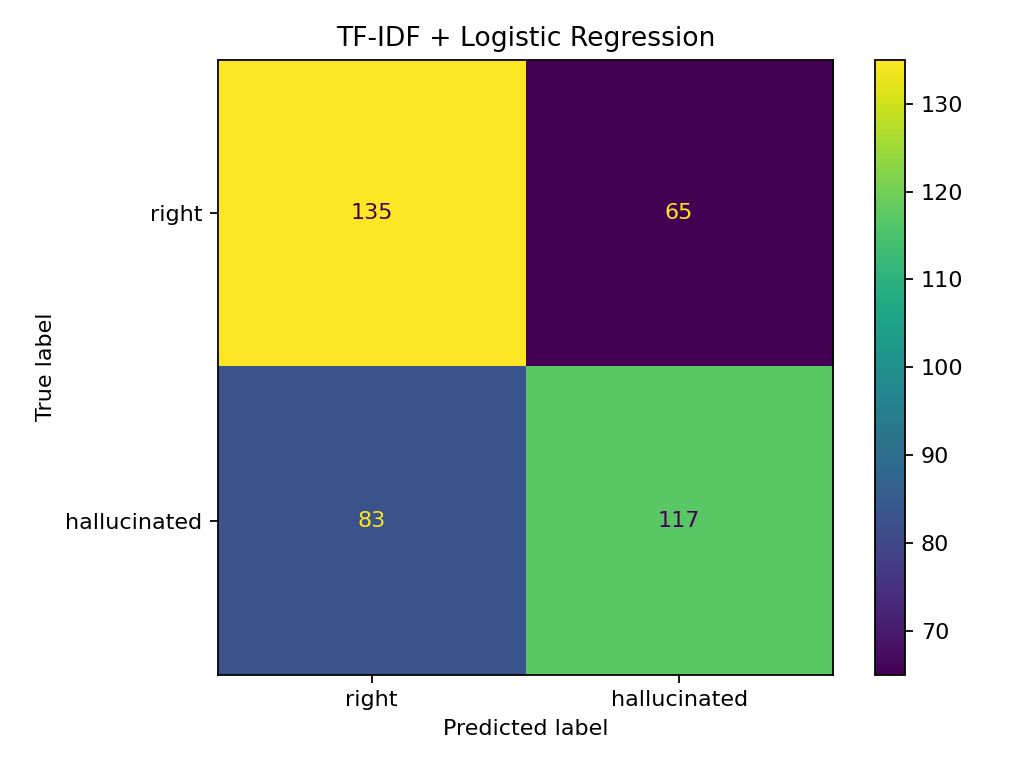
\includegraphics[width=0.42\linewidth]{figures/tf_idf_plus_logistic_regression_confusion.png}\hfill
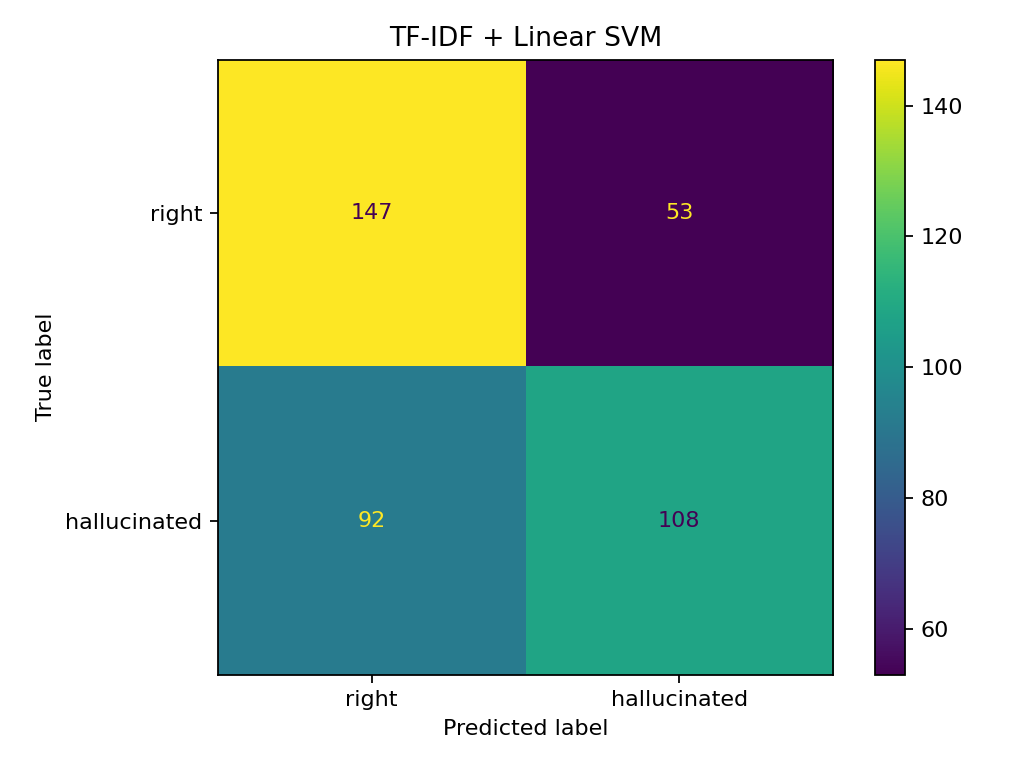
\includegraphics[width=0.42\linewidth]{figures/tf_idf_plus_linear_svm_confusion.png}
\caption{Confusion matrices for the two TF--IDF classifiers. Positive class is the hallucinated answer.}
\label{fig:confusion}
\end{figure}

\subsection{GPT-2 likelihood}
Table~\ref{tab:likelihood} presents the corrected likelihood metrics from the character-offset export. In the hypothesized direction, AUROC is 0.4437 and AUPRC is 0.4380. Reversing the score gives AUROC 0.5563 and AUPRC 0.5023. The reversed score is only weakly discriminative and does not establish that lower likelihood means hallucination. The balanced 200-instance evaluation has a baseline precision--recall average-precision reference near 0.5, so the reversed AUPRC is close to that baseline.
\begin{table}[H]
\centering
\caption{GPT-2 negative mean answer-token log-probability.}
\label{tab:likelihood}
\begin{tabular}{lrr}
\toprule
Score direction & AUROC & AUPRC\\
\midrule
Original (higher = more suspicious) & 0.4437 & 0.4380\\
Reversed & 0.5563 & 0.5023\\
\bottomrule
\end{tabular}
\end{table}

The corrected score summary is reported in the accompanying CSV rather than copied from the earlier likelihood export, because the initial and corrected exports use different token-selection implementations. The corrected metrics are the values used in this manuscript. Even with answer-token selection, a likelihood score remains a measure of model preference for a token sequence under the prompt, not a direct assessment of whether the answer is supported by the knowledge.

\section{Error Analysis and Discussion}
The classifier predictions and error-analysis CSVs are included in the repository so that examples can be inspected rather than relying only on aggregate metrics. A false positive is a right answer flagged as hallucinated; a false negative is a hallucinated answer predicted as right. These two error types have different practical consequences. A false positive may unnecessarily reject a correct answer, while a false negative allows an incorrect answer to pass the detector. The exported analysis labels these categories and preserves the source question, knowledge and answer for manual inspection.

The moderate classifier scores indicate that surface text and context contain signals associated with the benchmark labels, but the scores leave substantial error. The model may learn lexical patterns, answer length, phrasing or benchmark-generation artifacts. This is a plausible explanation rather than a demonstrated causal account; identifying such artifacts would require a dedicated analysis, such as controlling answer length or testing on a separate dataset. A stronger experiment would also report per-category error examples and test whether results persist across multiple random seeds.

GPT-2 likelihood performs poorly in the expected direction. This is consistent with the conceptual limitation that a language model can assign high probability to familiar but incorrect wording and low probability to an unusual correct answer. However, the current experiment does not isolate why the score fails. Prompt format, truncation, tokenization, the small sample and the construction of candidate answers may all matter. The reversed direction's AUROC of 0.5563 is close to chance and should not be presented as a useful detector.

\section{Threats to Validity and Limitations}
Several limitations constrain interpretation. First, the classifier results use a single group-based split, so estimates may be sensitive to which groups are held out. Repeated splits or cross-validation would better quantify variability. Second, the GPT-2 experiment includes only 100 pairs, which makes the ranking estimates uncertain. Third, HaluEval's benchmark labels and paired construction may introduce artifacts that are not representative of naturally occurring hallucinations. Fourth, the input combines knowledge, question and answer, so the classifier can exploit wording regularities and is not necessarily performing evidence-grounded fact checking.

Fifth, conditional token likelihood measures the probability of wording, not factuality. The score is sensitive to the prompt template, tokenization and truncation. Sixth, this project did not implement semantic entropy, sample multiple generations, cluster semantic equivalence classes, calibrate probabilities, or perform significance testing. Finally, no external held-out dataset was used. These limitations mean the findings should be read as exploratory evidence on a particular benchmark subset, not as a general claim about LLM hallucination detection.

\section{Conclusion and Future Work}
This study compared TF--IDF with Logistic Regression, TF--IDF with Linear SVM, and GPT-2 conditional candidate-answer likelihood on a small HaluEval QA sample. Linear SVM had the highest accuracy (0.6375), AUROC (0.7009) and AUPRC (0.7059), while Logistic Regression had higher recall and F1 at the selected threshold. Both classifiers showed modest discrimination. The corrected GPT-2 likelihood score had AUROC 0.4437 in the hypothesized direction and 0.5563 when reversed, providing little evidence that the score alone separates the two answer types.

Future work should use repeated group splits and confidence intervals, increase the likelihood sample, inspect error categories systematically, and evaluate on an independent dataset. A more faithful comparison with semantic uncertainty would require multiple generated answers and semantic-equivalence clustering. Claiming such a method as implemented would be inaccurate for this study. The main conclusion is therefore methodological: inexpensive lexical baselines provide a useful reference, while a single conditional-likelihood score is not sufficient to establish factual reliability in this experiment.

\section*{Research Integrity Note}
All numerical results in this manuscript are tied to the uploaded experiment CSVs. The corrected likelihood CSVs are preserved separately from the initial export so the analysis history remains visible. No confidence intervals, significance tests, or unrun experiments are claimed. Before submission, the author should verify all bibliographic metadata against the cited primary sources and ensure the course's AI-use disclosure requirements are met.

\begin{thebibliography}{9}
\bibitem{li2023halueval} J. Li, X. Cheng, W. X. Zhao, J.-Y. Nie, and J.-R. Wen. HaluEval: A Large-Scale Hallucination Evaluation Benchmark for Large Language Models. In \emph{Proceedings of EMNLP}, pages 6449--6464, 2023. doi:10.18653/v1/2023.emnlp-main.397.
\bibitem{farquhar2024semantic} S. Farquhar, J. Kossen, L. Kuhn, and Y. Gal. Detecting Hallucinations in Large Language Models Using Semantic Entropy. \emph{Nature}, 630:625--630, 2024. doi:10.1038/s41586-024-07421-0.
\bibitem{vashurin2025polygraph} R. Vashurin et al. Benchmarking Uncertainty Quantification Methods for Large Language Models with LM-Polygraph. \emph{Transactions of the Association for Computational Linguistics}, 13, 2025. doi:10.1162/tacl_a_00737.
\bibitem{ravichander2025halogen} S. Ravichander et al. HALoGEN: Fantastic LLM Hallucinations and Where to Find Them. In \emph{Proceedings of ACL}, 2025. doi:10.18653/v1/2025.acl-long.71.
\bibitem{rucaiboxhalueval} RUCAIBox. HaluEval: A Large-Scale Hallucination Evaluation Benchmark for Large Language Models. Dataset repository. \url{https://github.com/RUCAIBox/HaluEval} (accessed October 2026).
\end{thebibliography}
\end{document}
